\documentclass{beamer}
\usepackage[utf8]{inputenc}
\usepackage[slovene,english]{babel}
\usepackage{verbatim}

\usetheme{default}

\title{Vrtače dinarskega krasa}

% A subtitle is optional and this may be deleted
% \subtitle{Optional Subtitle}

\author{Rok Mihevc \\ Mentor: prof. Rudolf Podgornik}

\institute[Univerza v Ljubljani]
{
\begin{center} 
  
\includegraphics[width=0.4\textwidth]{slike/logo_fmf_uni-lj_sl.pdf} 
\end{center}
}

\date{Ljubljana, 2014}


% Delete this, if you do not want the table of contents to pop up at
% the beginning of each subsection:
%\AtBeginSubsection[]
%{
%  \begin{frame}<beamer>{Outline}
%    \tableofcontents[currentsection,currentsubsection]
%  \end{frame}
%}


\begin{document}

\begin{frame}
  \titlepage
\end{frame}

\begin{frame}{Pregled}
  \tableofcontents
  % You might wish to add the option [pausesections]
\end{frame}


\section{Preučevanje realnih vrtač}

\subsection{Realne vrtače}

\begin{frame}{Kraške vrtače}{So zaprte koncentrične depresije}
\begin{center} 
  \hspace*{-0.075\textwidth}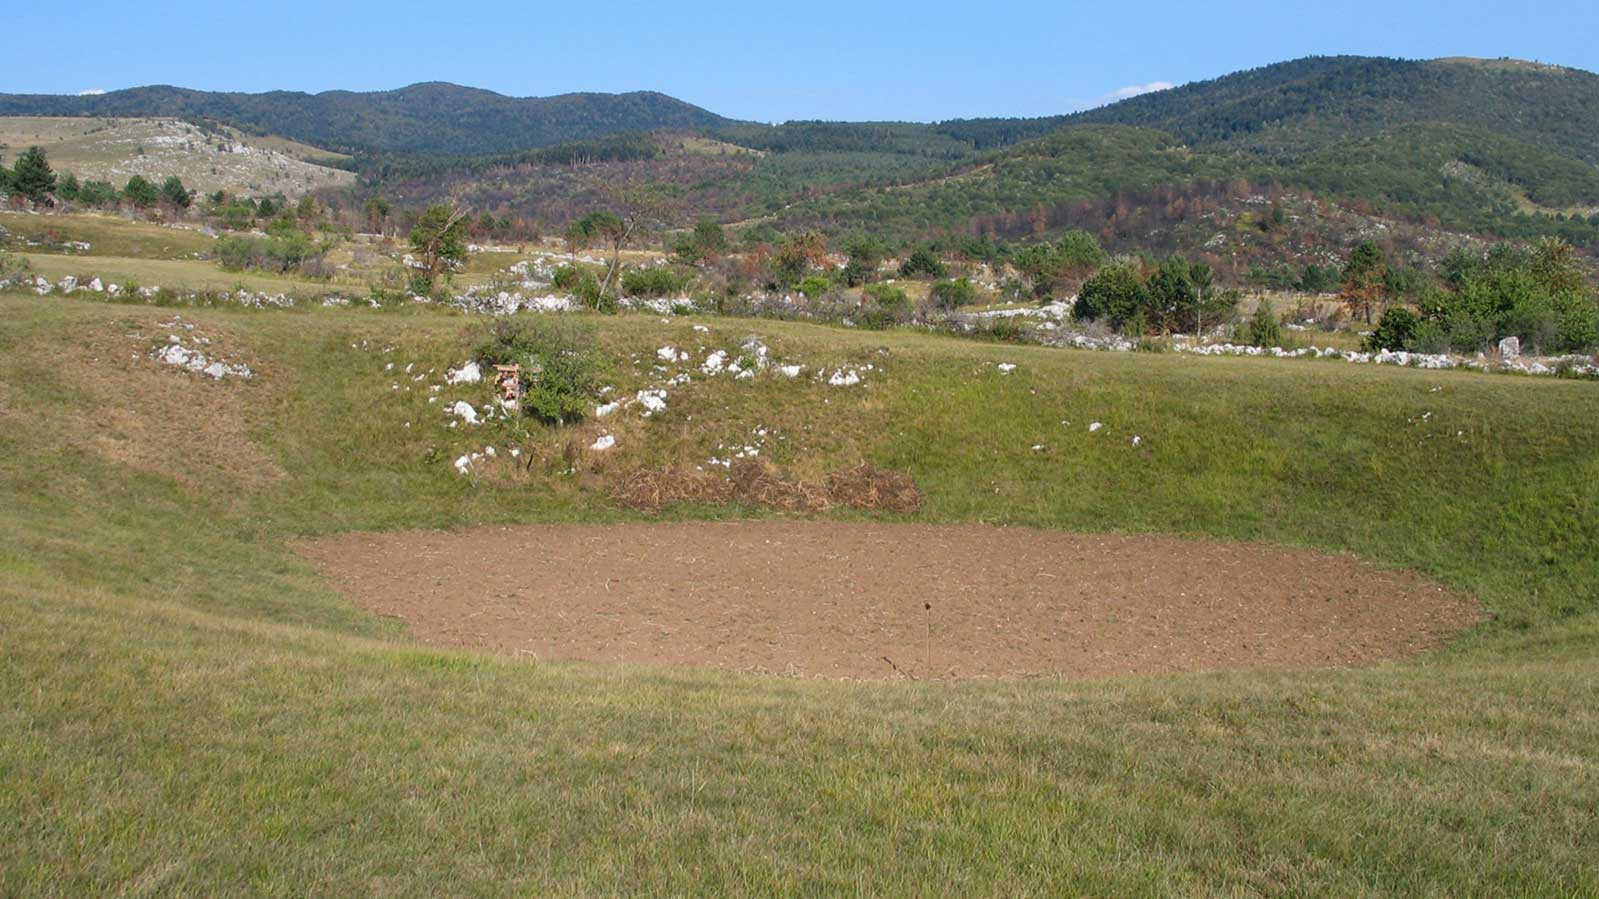
\includegraphics[width=1.15\textwidth]{slike/vrtaca} \\
  Jurišče, Slovenija
\end{center} 
\end{frame}

\begin{frame}{Kraške vrtače}{Najdemo jih na starih kraških poljih in planotah}
  \begin{center}
    \hspace*{-0.075\textwidth}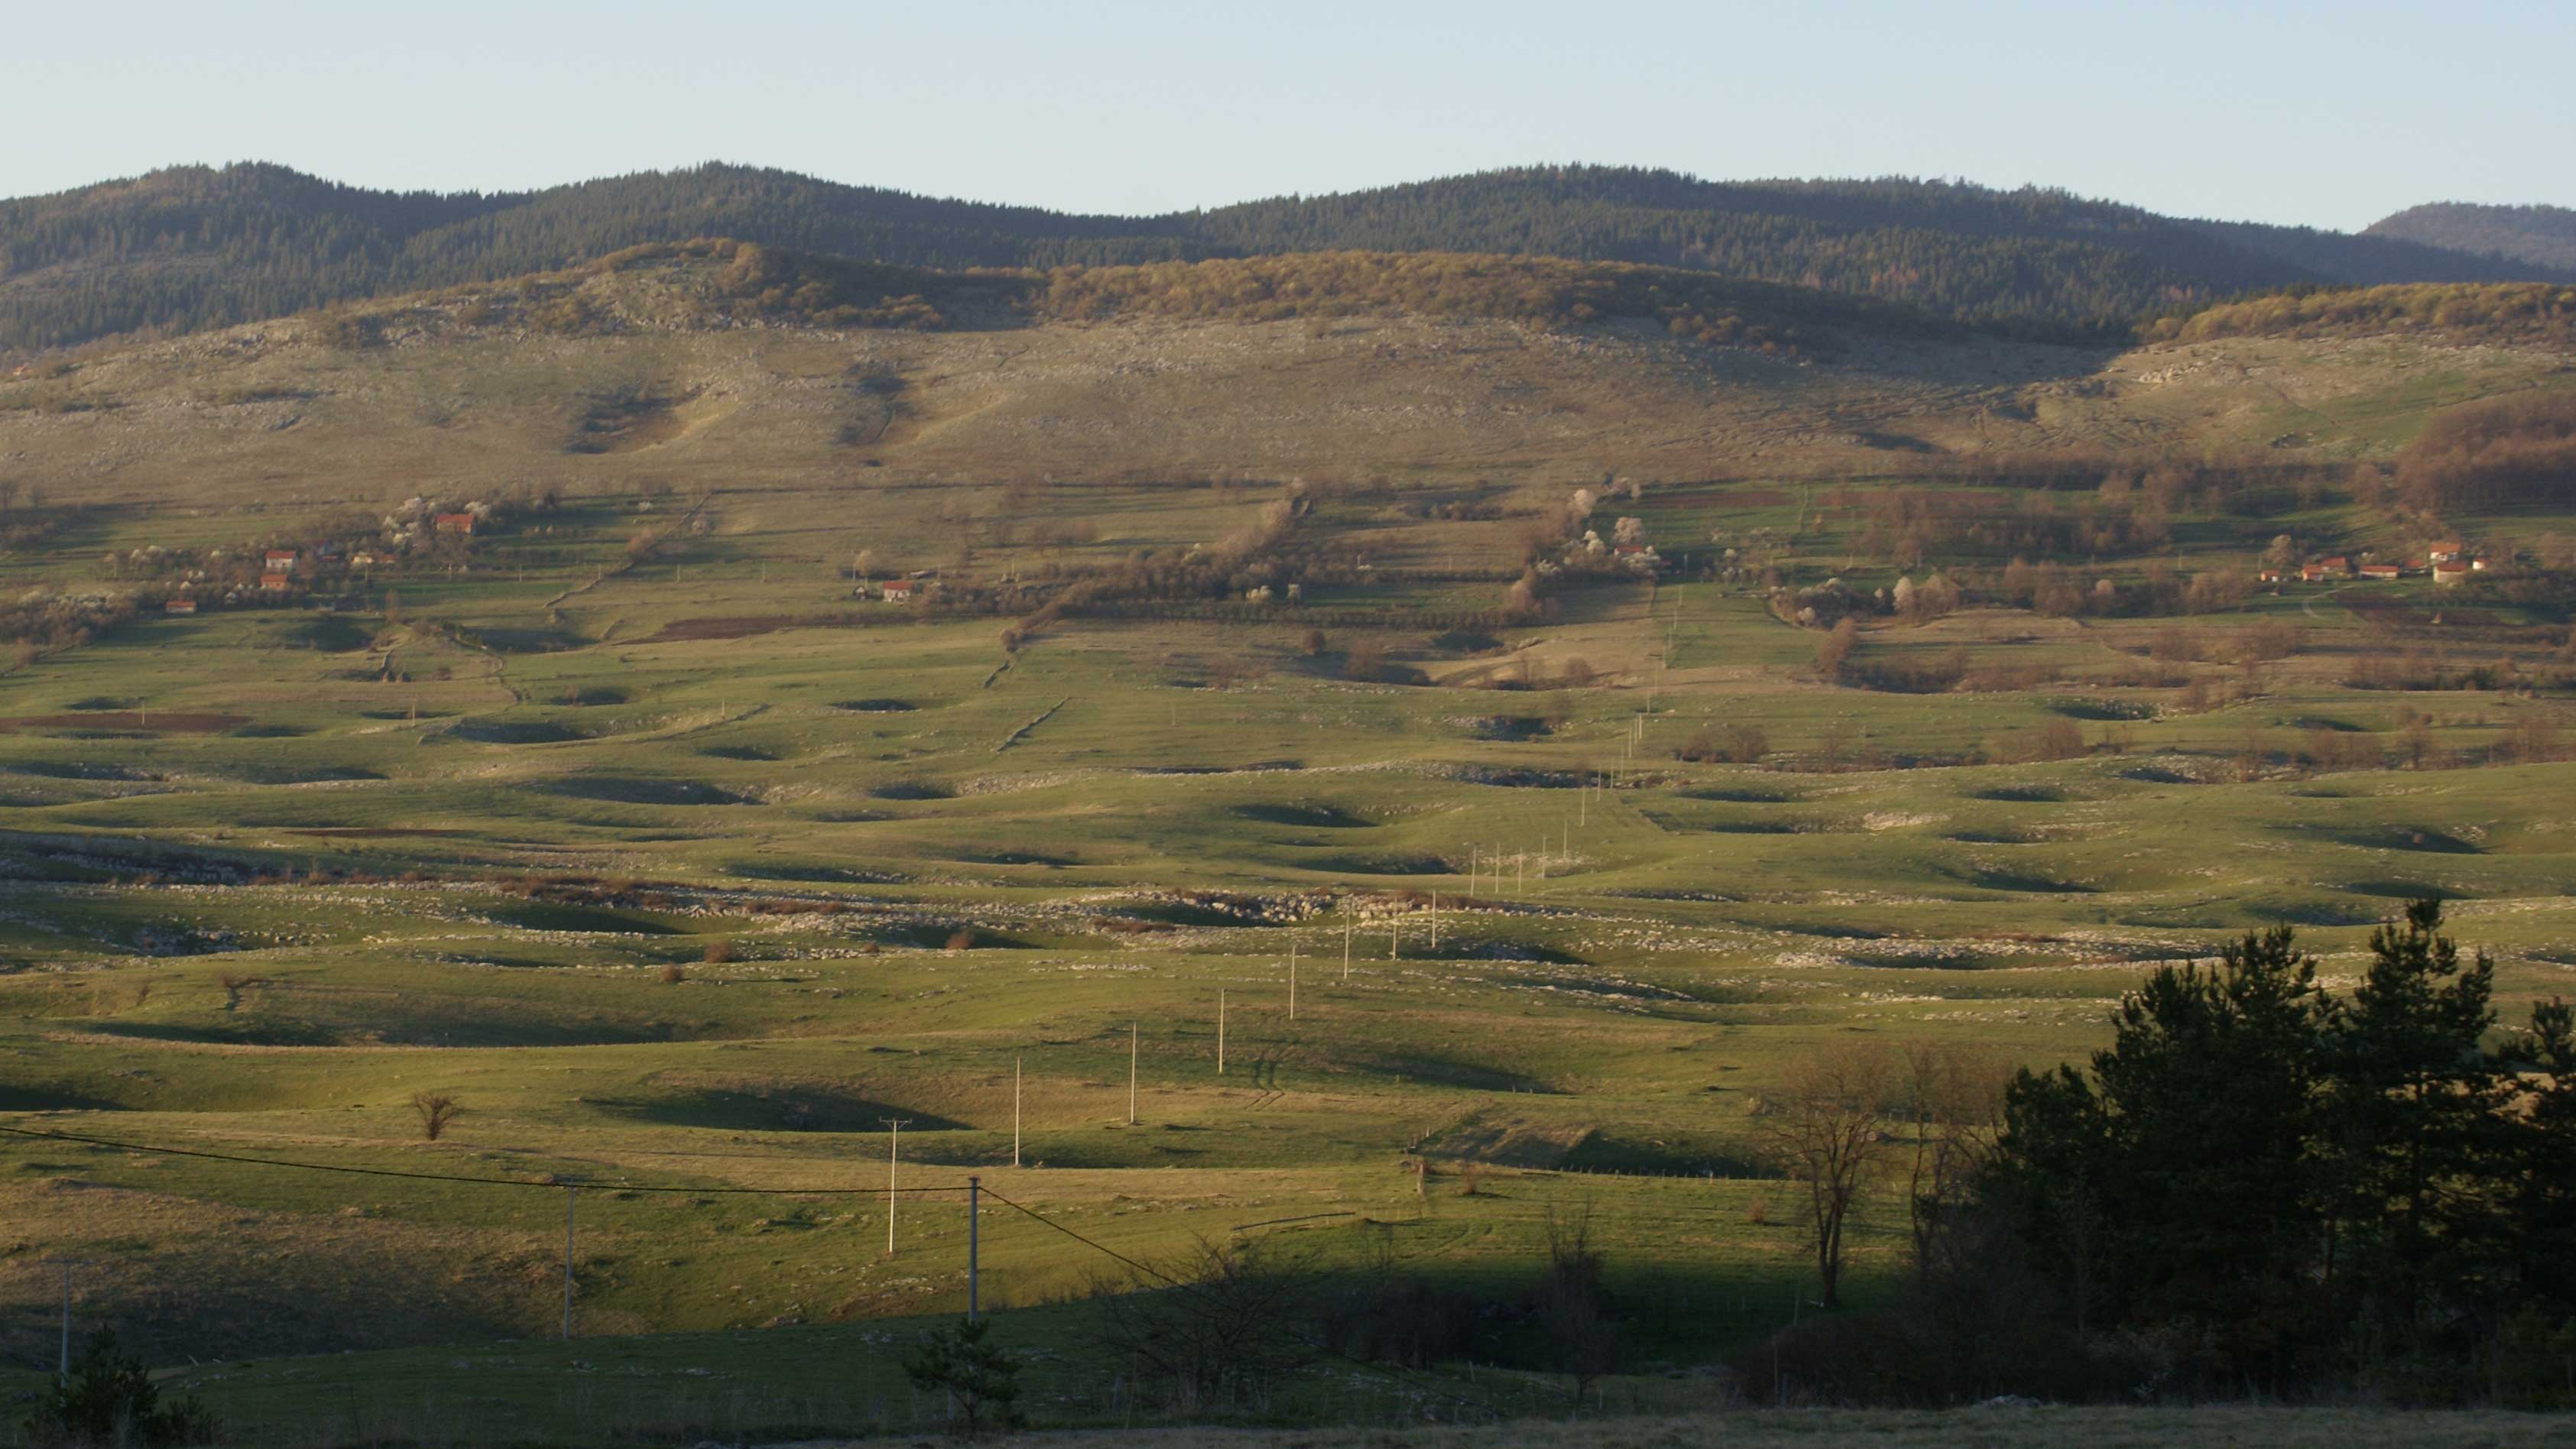
\includegraphics[width=1.15\textwidth]{slike/bpetrovac} \\
    Kapljuh, BiH
  \end{center}
\end{frame}

\begin{frame}{Kraške vrtače}{Več predlaganih modelov nastanka}
  \begin{center}
    \hspace*{-0.075\textwidth}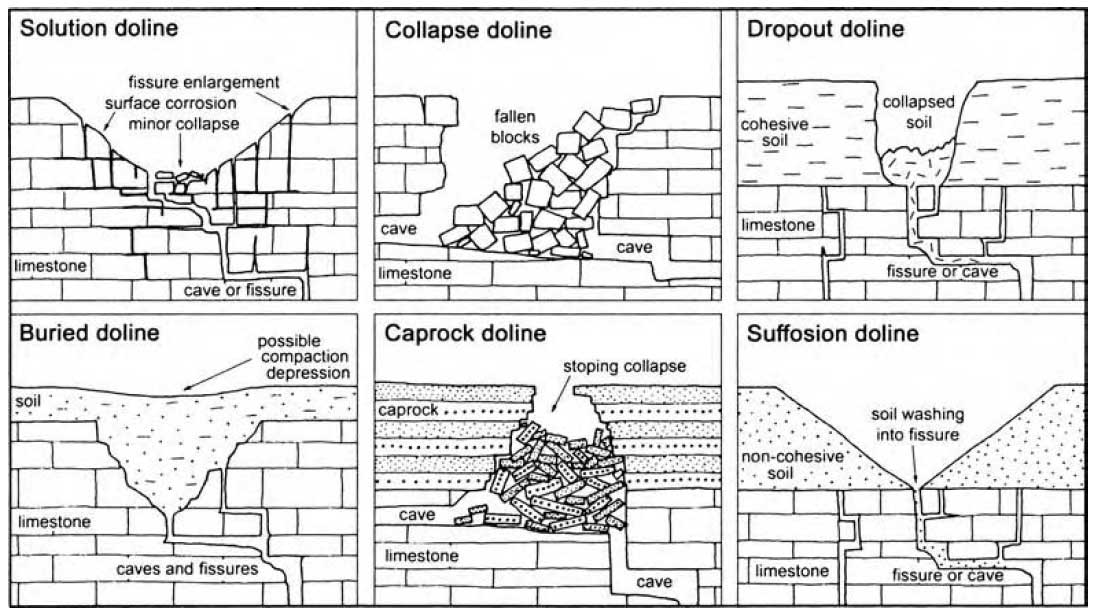
\includegraphics[width=1.15\textwidth]{slike/nastanek}
  \end{center}
\end{frame}

\begin{comment}
\begin{frame}{Kraške vrtače}{Več predlaganih modelov nastanka}
  \begin{center}
    \hspace*{-0.1\textwidth}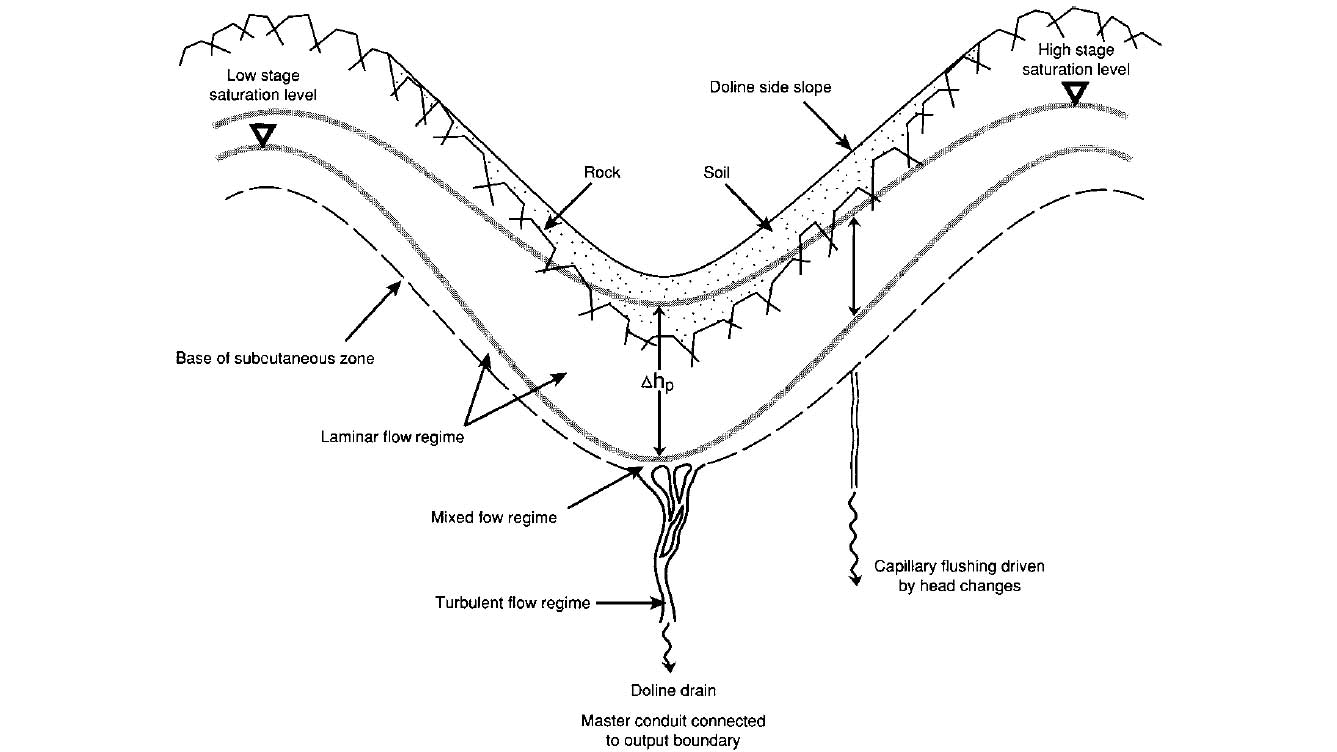
\includegraphics[width=1.2\textwidth]{slike/nastanek2}
  \end{center}
\end{frame}
\end{comment}

\begin{frame}{Kraške vrtače}{Ni podrobnejših študij procesov, ki jih oblikujejo}

\begin{columns}
  \begin{column}{0.6\textwidth}
    
\includegraphics[width=\textwidth]{slike/vrtaca-ford-williams.png}
  \end{column}

  \begin{column}{0.5\textwidth}
    \includegraphics[width=\textwidth]{slike/verd}
  \end{column}
\end{columns}
\end{frame}


\subsection{LiDAR}

% You can reveal the parts of a slide one at a time
% with the \pause command or \item<3-> 

\begin{frame}{LiDAR}{Posnetek območja Menišije, ločljivost $1m^2$}
\begin{center}
  \hspace*{-0.95cm}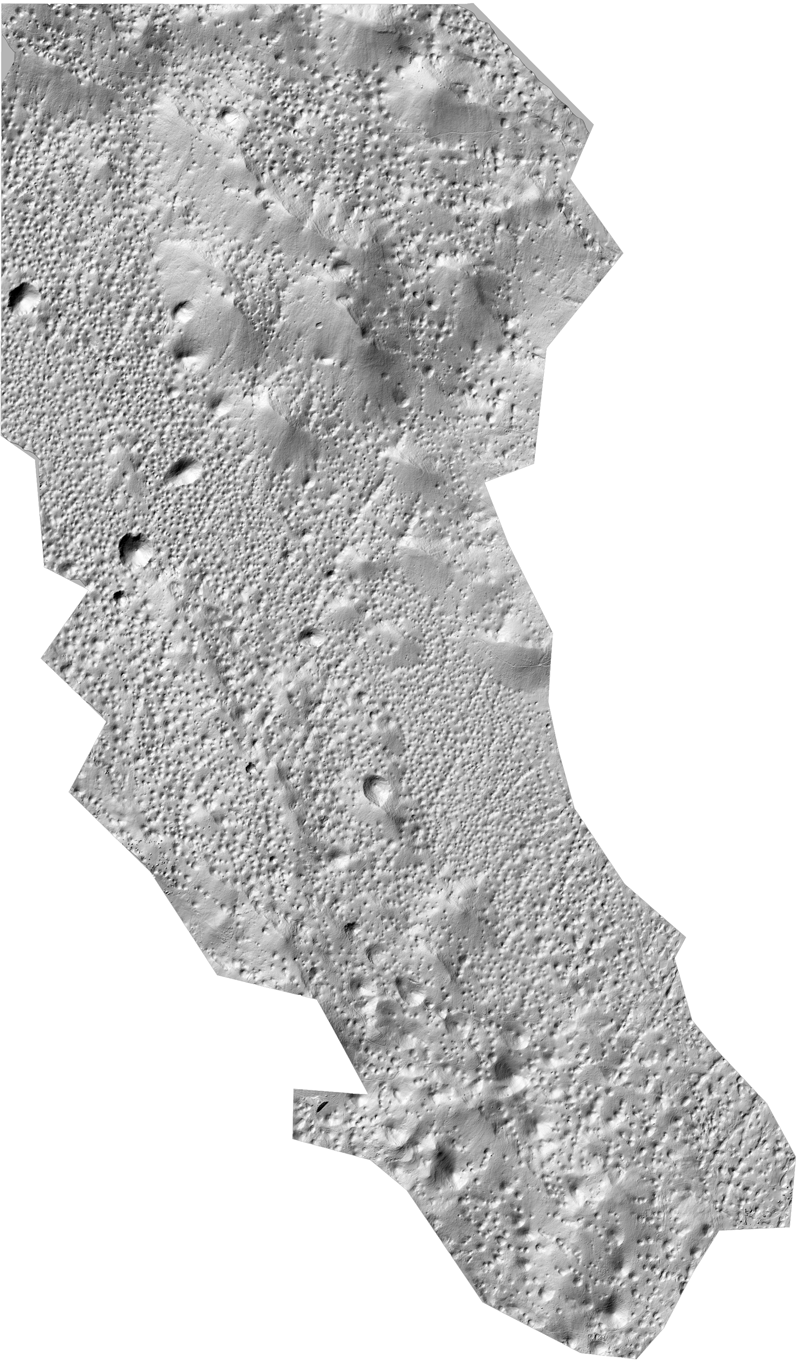
\includegraphics[width=0.7\textwidth,angle=90]{slike/menisija-relief}
\end{center}
\end{frame}

\begin{frame}{Računalniški vid}{Identificiramo konkavnosti v reliefu in jih označimo}
\begin{columns}
  \begin{column}{0.55\textwidth}
    \hspace*{0.02\textwidth}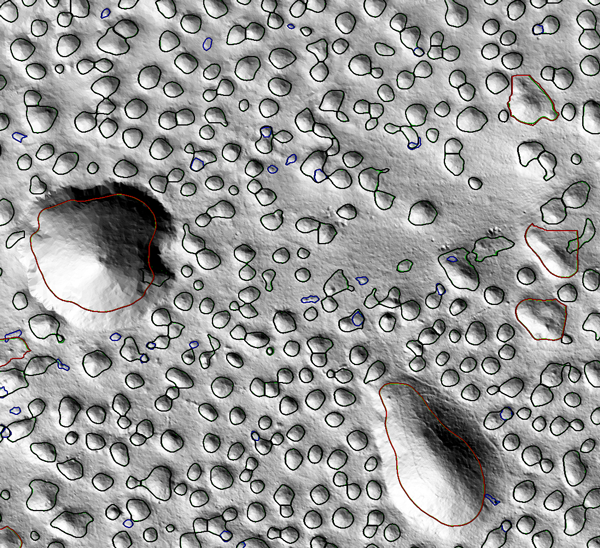
\includegraphics[width=\textwidth]{slike/menisija-vrtace}
  \end{column}

  \begin{column}{0.7\textwidth}
    \hspace*{-0.025\textwidth}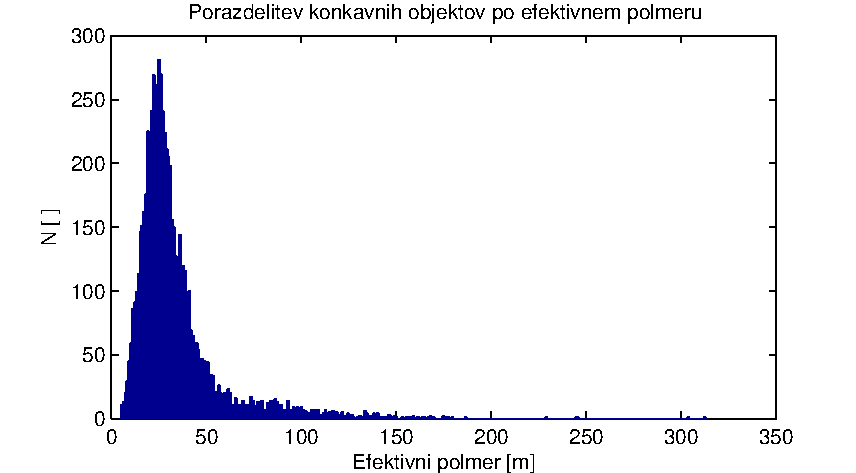
\includegraphics[width=\textwidth]{slike/menisija-polmeri-hist}
    \footnotesize
    \[ A = \sum piksli\]
    \[ r_{eff} = \sqrt{\frac{A}{\pi}} \]
  \end{column}
\end{columns}
\end{frame}

\begin{frame}{Povprečimo konkavnosti}{Dobimo 'povprečno vrtačo', prilegamo gaussovko na vse najdene konkavnosti}

\begin{columns}
  \begin{column}{0.5\textwidth}
    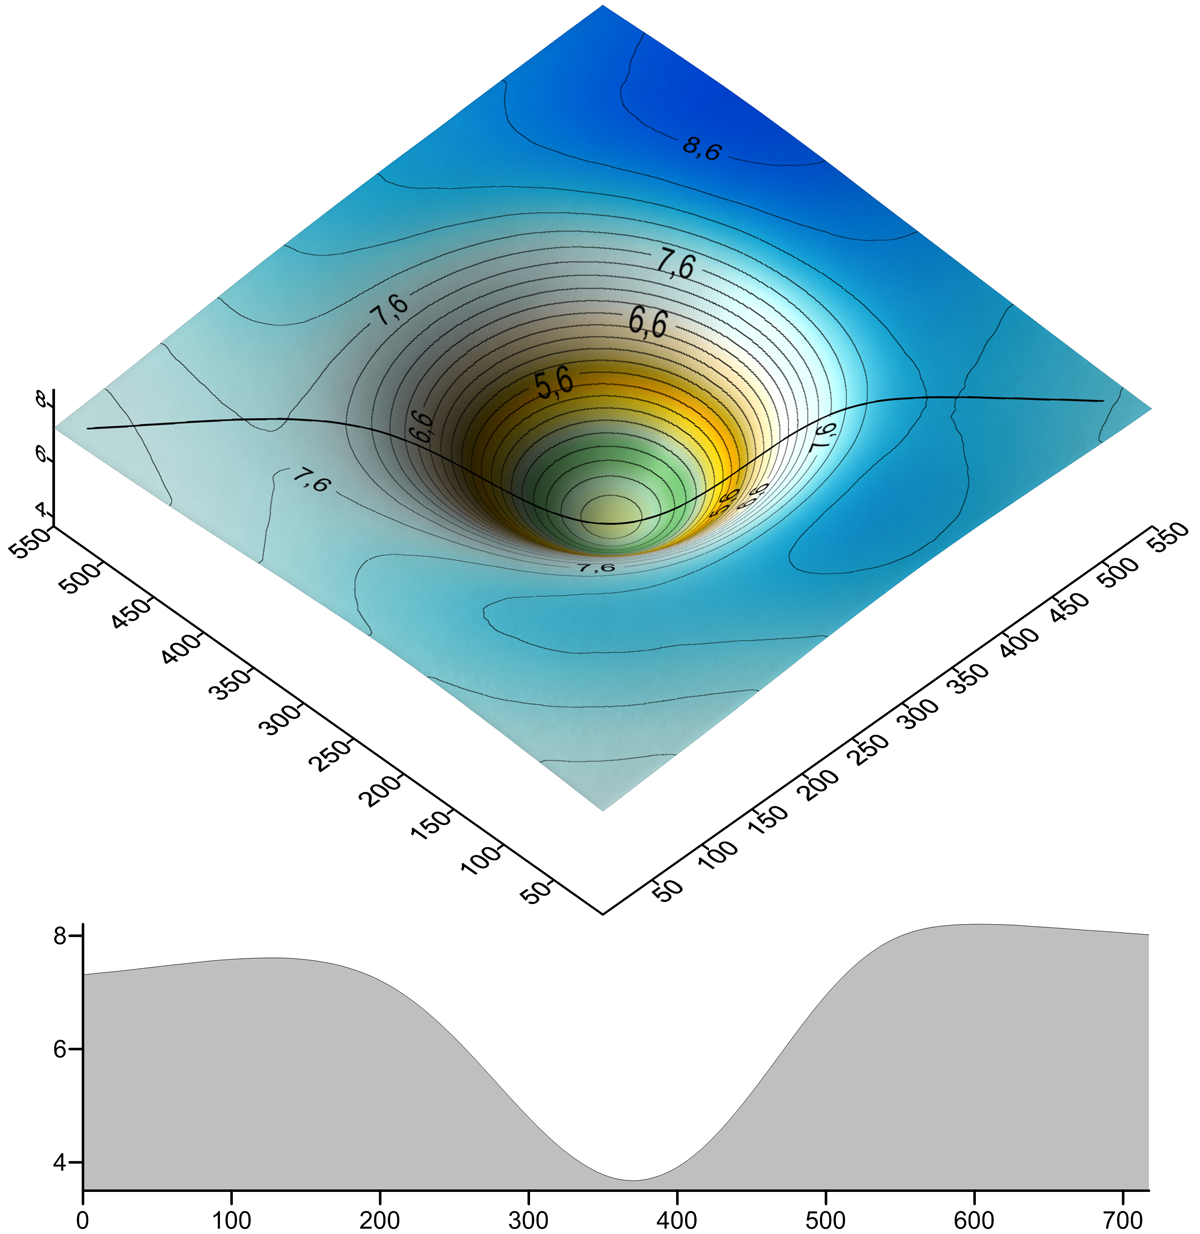
\includegraphics[width=\textwidth]{slike/menisija-vrtaca}
    \begin{equation} \resizebox{.75\textwidth}{!}{ $f(r) = A \cdot e^{-\frac{(r-r_0)^2}{\sigma^2}} + C$} \end{equation}
  \end{column}

  \begin{column}{0.45\textwidth}
    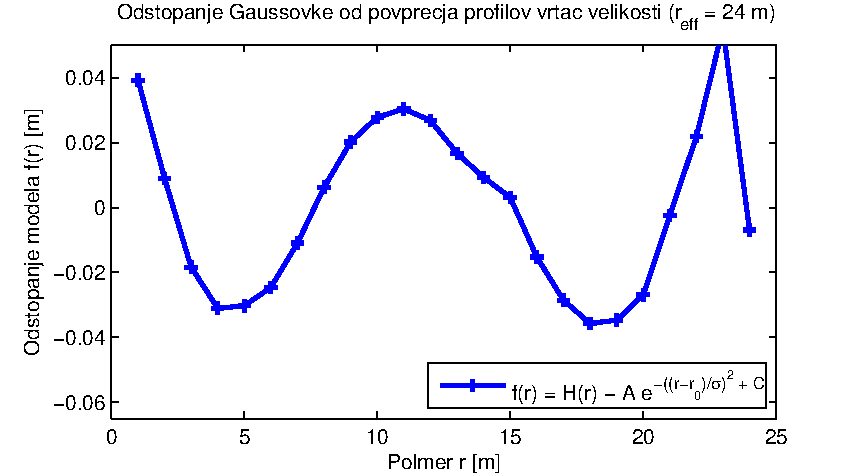
\includegraphics[width=\textwidth]{slike/menisija-profil-21-fit} \\
    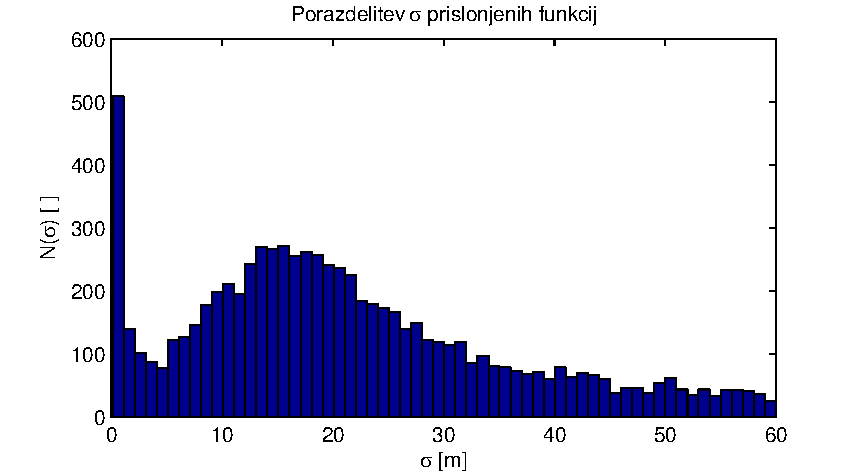
\includegraphics[width=\textwidth]{slike/menisija-sigme-hist} \\
    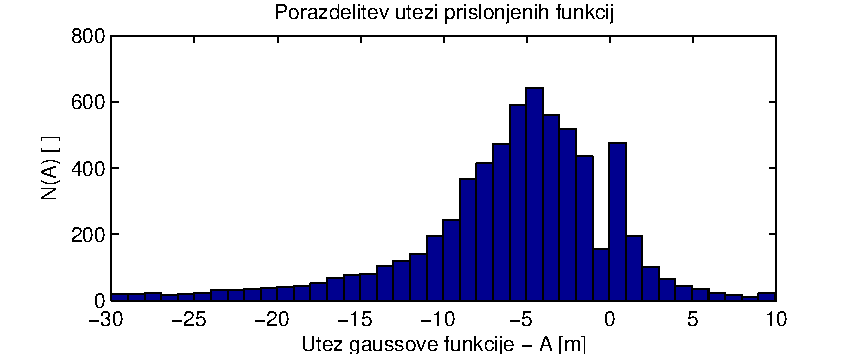
\includegraphics[width=\textwidth]{slike/menisija-globine-hist}
  \end{column}
\end{columns}

\end{frame}


\section{Rast vmesnikov}

\subsection{Definicije}

\begin{frame}{Rast vmesnikov}{Širina vmesnika, priraščanje}
\begin{columns}
  \begin{column}{0.45\textwidth}
     \hspace*{-0.05\textwidth}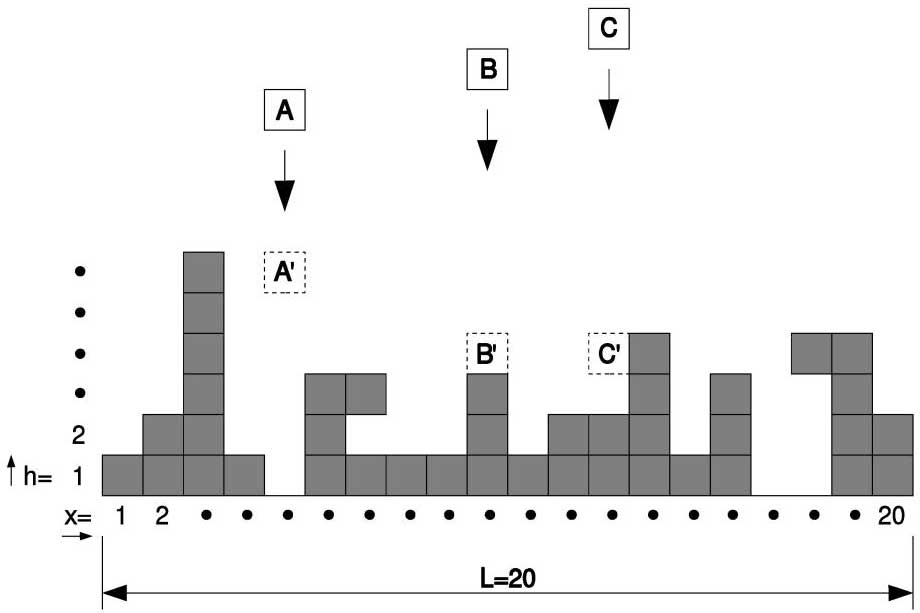
\includegraphics[width=1.1\textwidth]{slike/bdep}
  \end{column}

  \begin{column}{0.55\textwidth}
    \footnotesize
    \begin{equation} \bar{h} = \frac{1}{L} \sum_{i=1}^L h(i,t) \end{equation}
    \newline
    \begin{equation} w(L,t) = \sqrt{\frac{1}{L} \sum_{i=1}^L (h(i,t)-\bar{h}(t))^2} \end{equation}
    \newline
    \begin{equation} \bar{h}(t) \sim t \end{equation}
  \end{column}
\end{columns}
\end{frame}


\begin{frame}{Rast vmesnikov}{Povprečna širina vmesnika v času, eksponent hrapavosti}
\begin{center}
  \footnotesize
  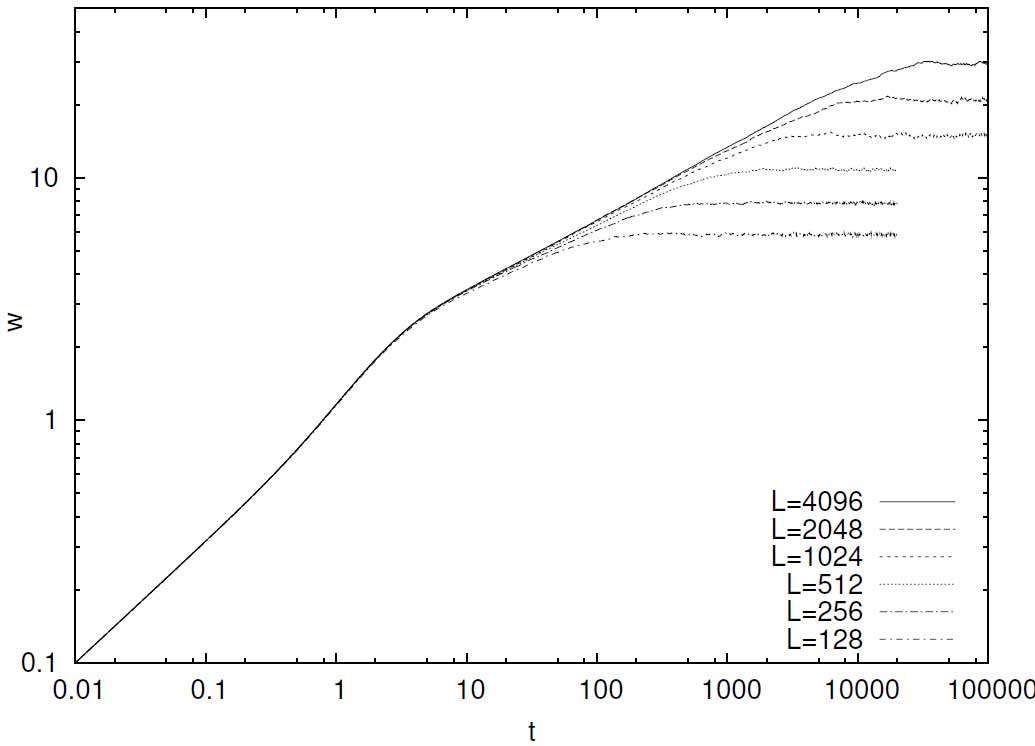
\includegraphics[width=0.8\textwidth]{slike/sirine-vmesnika}

\begin{columns}
  \begin{column}{0.6\textwidth}
    \begin{equation} w(L,t) = \left\langle \sqrt{\frac{1}{L} \sum_{i=1}^L (h(i,t)-\bar{h}(t))^2} \right\rangle \end{equation}
  \end{column}
  \begin{column}{0.4\textwidth}
    \begin{equation} w_{sat}(L) \sim L^\alpha \end{equation}
  \end{column}
\end{columns}
\end{center}
\end{frame}


\subsection{Rezultati}

\begin{frame}{Rast vmesnikov}{Zasičeni režim, hrapavost Menišije}
\begin{center}
  \footnotesize
  \hspace*{-0.04\textwidth}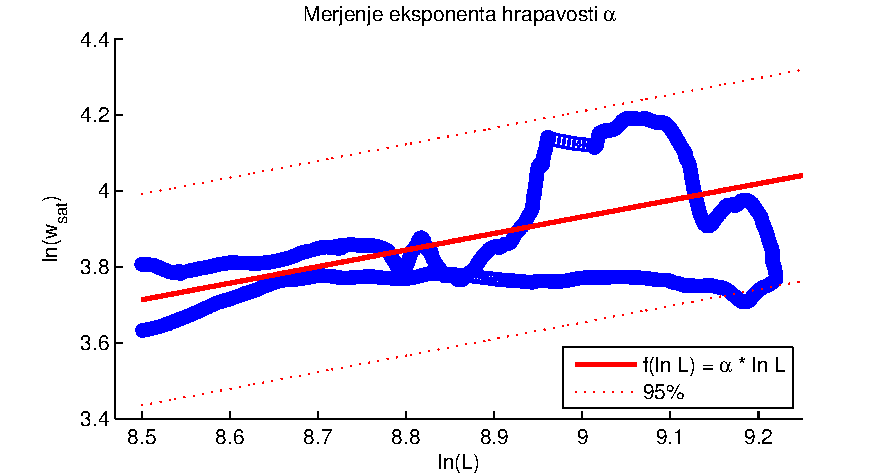
\includegraphics[width=1.1\textwidth]{slike/menisija-alfa}
  \begin{equation} \alpha = \frac{\partial ( ln (w_{sat}) ) }{\partial ( ln L )} =  0.4368 \pm 0.0005 \end{equation}
\end{center}
\end{frame}


\section{Modeliranje}

\subsection{Kardar-Parisi-Zhang}

\begin{frame}{Kardar-Parisi-Zhang}{Stohastična difuzijska enačba, teoretično napovedana hrapavost}
\begin{center}
  \footnotesize
  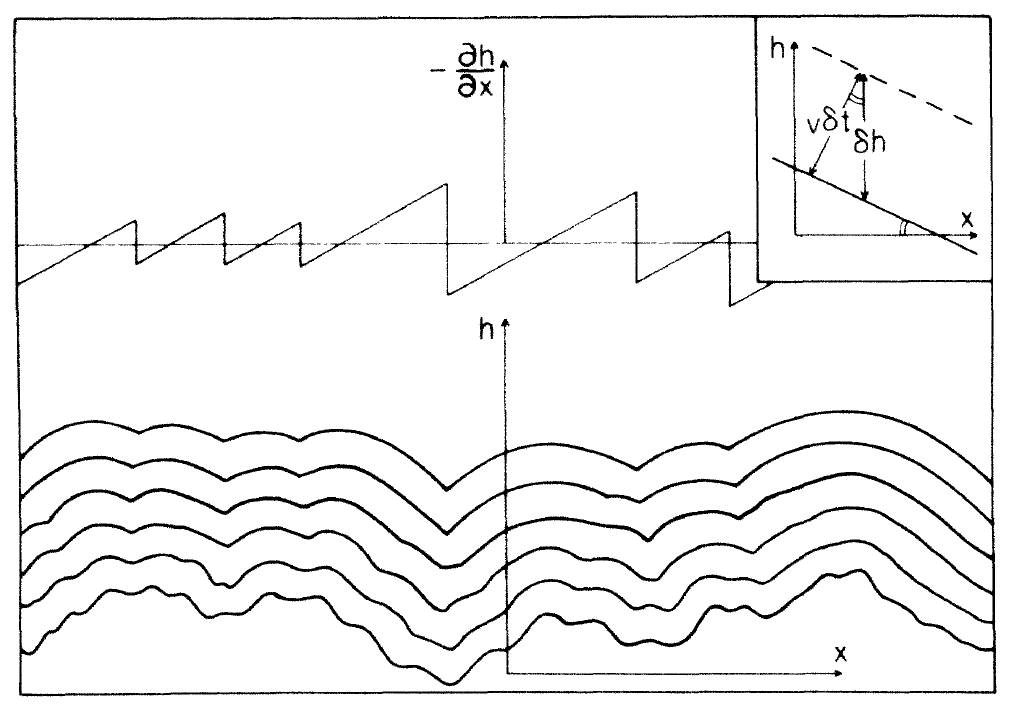
\includegraphics[width=0.7\textwidth]{slike/kpz}
  \begin{equation} \frac{\partial h}{\partial t} = \nu \nabla^2 h + \frac{\lambda}{2} (\nabla h)^2 + \eta (\mathbf{x},t) \end{equation}
  \begin{equation} \langle \eta(\mathbf{x},t) \eta(\mathbf{x'},t')\rangle = \delta(\mathbf{x}-\mathbf{x'})(t-t') \end{equation}
  Napove: $\alpha = \frac{1}{2}$
\end{center}
\end{frame}


\begin{frame}{Kardar-Parisi-Zhang}{Simulacija}
\begin{center}
  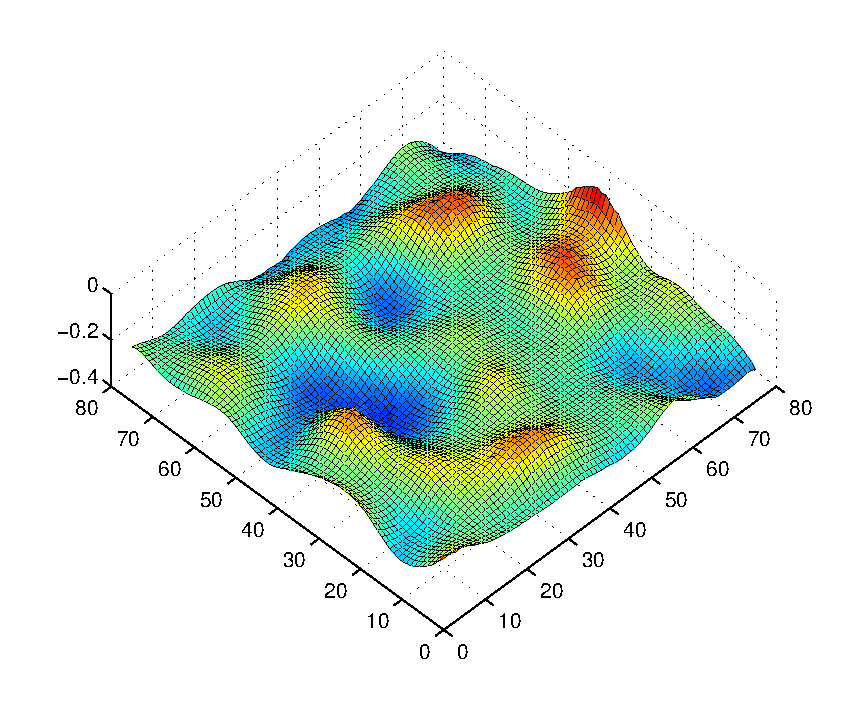
\includegraphics[width=.95\textwidth]{slike/KPZ-numericno}
\end{center}
\end{frame}


\subsection{Dinamične enačbe}

\begin{frame}{Dinamične enačbe}{Primer: Logistična rast}
\begin{block}{Model}
  Rast v času je odvisna od višine in razdalje do nosilne kapacitete
  \begin{equation} \frac{\partial h(t)}{\partial t} = a \cdot \left( 1 - \frac{h(t)}{K} \right) h(t) \end{equation}
\end{block}
\begin{block}{Rešitev}
  \begin{equation} h(t) = \frac{h_0 K e^{a t}}{K + h_0 (e^{a t}-1)} \end{equation}
\end{block}
\end{frame}

\begin{frame}{Dinamične enačbe}{Primer: Logistična rast}
\begin{center}
  \hspace*{-0.09\textwidth}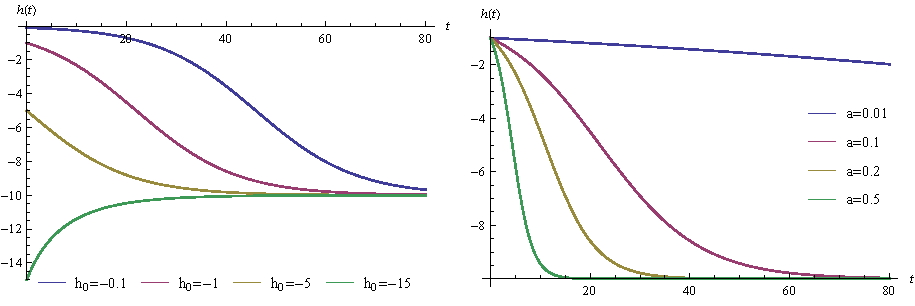
\includegraphics[width=1.2\textwidth]{slike/logisticna-rast}
  \footnotesize
\begin{columns}
  \begin{column}{0.5\textwidth}
  \[ K = 10 \]
  \[ a = 0.1 \]
  \end{column}
  \begin{column}{0.5\textwidth}
  \[ K = 10 \]
  \[ h_0 = 0.1 \]
  \end{column}
\end{columns}
\end{center}
\end{frame}

\subsection{Difuzijsko dinamične enačbe}

\begin{frame}{Difuzijsko dinamične enačbe}{Primer: Difuzijska logistična rast}
\begin{block}{Model}
  Fisher-Kolmogorov-a enačba, rešitev iščemo numerično
  \begin{equation} \frac{ \partial h(t,x) }{ \partial t} = D \Delta h(t,x) + a \cdot h(t,x) \cdot (1 - \frac{h(t,x)}{K}) \end{equation} 
\end{block}
\begin{block}{Robni pogoji}
        \begin{equation}
          \begin{aligned}
            h(0,x) =  - e^{-x^2}, x \in D \\
            h(t,x) = 0, x \in \partial D \\
            \frac{\partial h(t,x)}{\partial n} = 0, x \in \partial D \\
          \end{aligned}
        \end{equation}
\end{block}
\end{frame}

\begin{frame}{Difuzijsko dinamične enačbe}{Primer: Difuzijska logistična rast}
\begin{columns}
  \begin{column}{0.8\textwidth}
    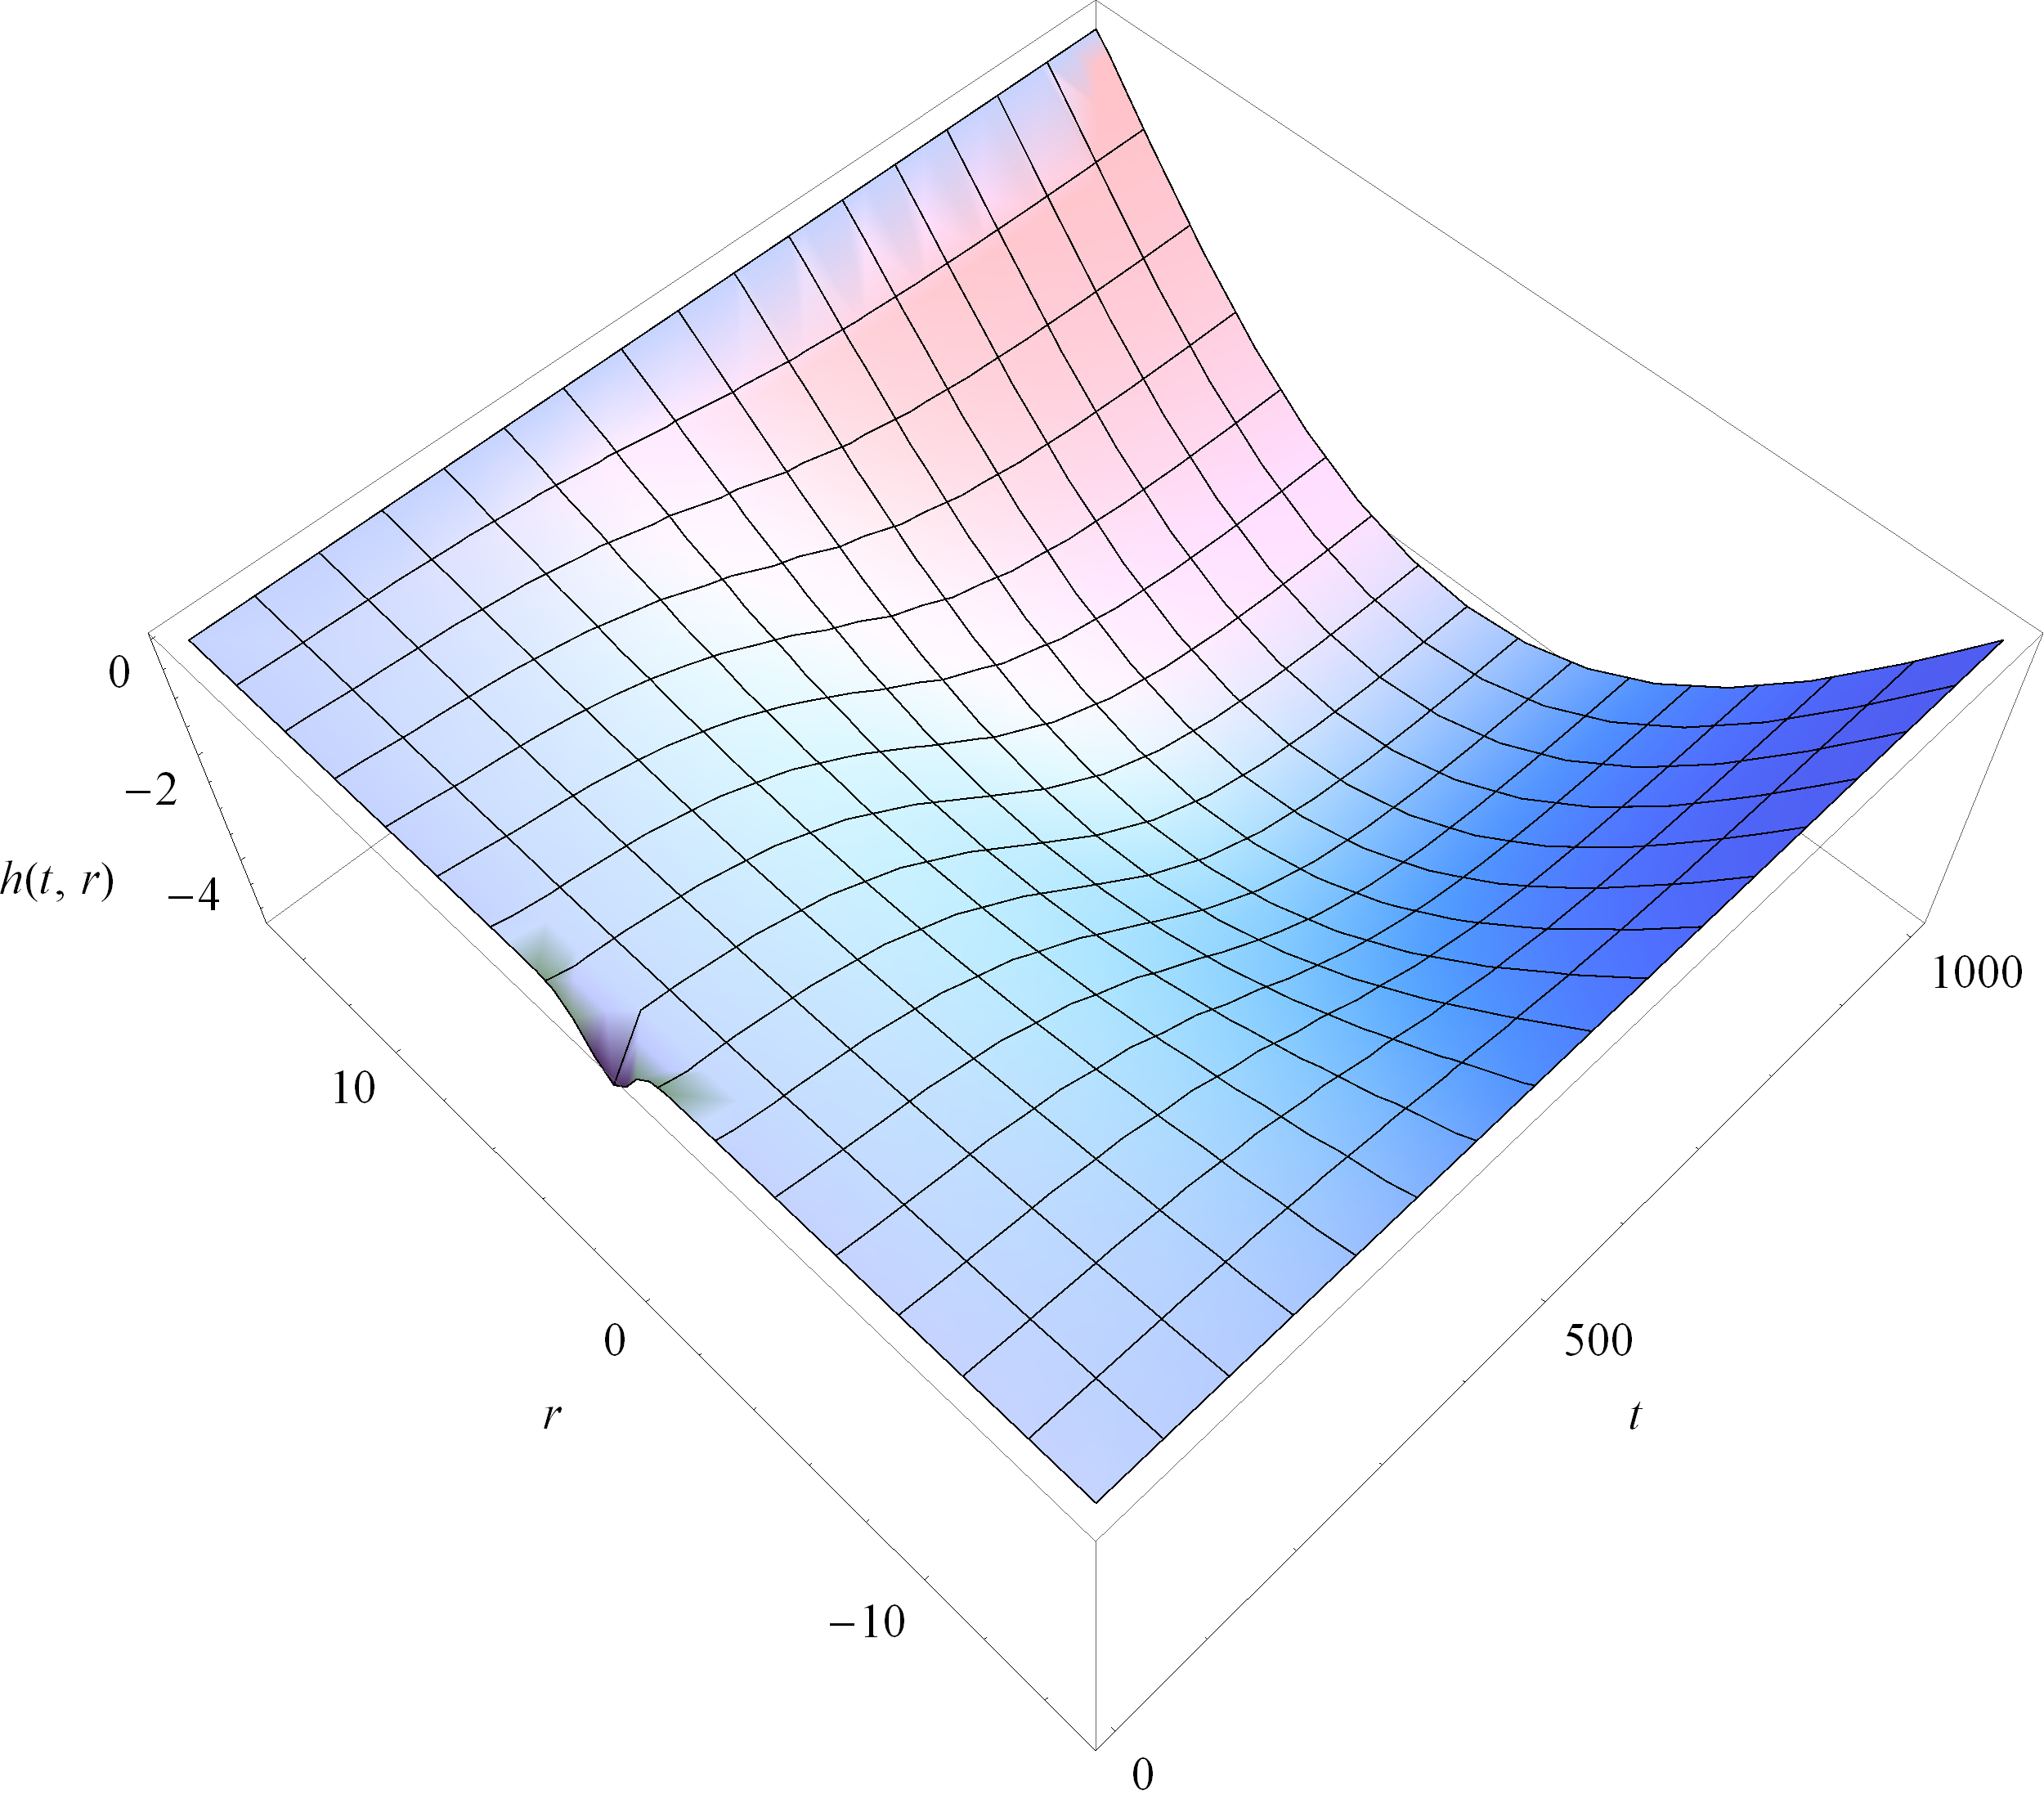
\includegraphics[width=1.05\textwidth]{slike/difuzija-logisticna-rast2.png}
  \end{column}
  \begin{column}{0.3\textwidth}
    \footnotesize
    \[ D = 1 \]
    \[ a = \frac{1}{50} \]
    \[ K = -10 \]
  \end{column}
\end{columns}
\end{frame}


% Placing a * after \section means it will not show in the
% outline or table of contents.
\section*{Zaključek}

\begin{frame}{Povzetek}
  \begin{itemize}
  \item<1->
    Segmentacija in analiza vrtač na digitalnem reliefu je relativno enostavna naloga
  \item<2->
    Vrtače so približno Gaussove oblike
  \item<3->
    Kardar-Parisi-Zhang-ova rast površja napove podobno hrapavost, kot jo opazimo v Menišiji
  \item<4->
    Izbira fizikalnega modela je zaradi pomanjkanja informacij o dinamiki težka
    \begin{itemize}
      \item<5->
        Najmanj napačen se zdi model logistične difuzijske rasti
    \end{itemize}
    \item<6->
      Natančnejši geološki študij dinamike reliefa bi bil v pomoč
  \end{itemize}
\end{frame}


\begin{comment}
\appendix
\section<presentation>*{\appendixname}
\subsection<presentation>*{Bibliografija}

\begin{frame}[allowframebreaks]
  \frametitle<presentation>{Bibliografija}
    
  \begin{thebibliography}{10}
    
  \beamertemplatebookbibitems
  % Start with overview books.

  \bibitem{Author1990}
    A.~Author.
    \newblock {\em Handbook of Everything}.
    \newblock Some Press, 1990.
 
    
  \beamertemplatearticlebibitems
  % Followed by interesting articles. Keep the list short. 

  \bibitem{Someone2000}
    S.~Someone.
    \newblock On this and that.
    \newblock {\em Journal of This and That}, 2(1):50--100,
    2000.
  \end{thebibliography}
\end{frame}

\end{comment}

\end{document}


